
%\chapter{Week5}

\section{Friday}\index{week5_Friday_lecture}
This lecture has two goals. The first is to see \emph{how orthogonality makes it easy to find the projection matrix $\bm P$ and the projection $\Proj_{\mathcal{C}(\bm A)}\bm b$}. The key idea is that \textit{Orthogonality makes the product $\bm A\trans\bm A$ a diagonal matrix}. The second goal is to \emph{show how to construct orthogonal basis of $\mathcal{C}(\bm A)$}. For matrix $\bm A=\begin{bmatrix}
a_1&a_2&\dots&a_n
\end{bmatrix}$, the columns may not be orthogonal. We intend to convert $a_1,\dots,a_n$ to orthogonal vectors, which will be the columns of a new matrix $\bm Q$.

\subsection{Orthonormal basis}
The vectors $\bm q_1,\dots,\bm q_n$ are \emph{orthogonal} when their inner product $\inp{\bm q_i}{\bm q_j}$ are zero. ($i\ne j$.) With one more step--each vector is just divided by its length, then the collection of vectors become \emph{orthogonal unit vectors}. Their lengths are all 1. Then this basis is called \emph{orthonormal}.
\begin{definition}[orthonormal]
The collection of vectors $\bm q_1,\dots,\bm q_n\in\mathbb{R}^m$ is said to be:
\begin{itemize}
\item
\emph{orthogonal} if $\inp{\bm q_i}{\bm q_j}=0$ for all $i,j$ with $i\ne j$
\item
\emph{orthonormal} if $\|\bm q_i\|_2=1$ for all $i$ and $\inp{\bm q_i}{\bm q_j}=0$ for all $i,j$ with $i\ne j$, or equivalently, 
\[
\inp{\bm q_i}{\bm q_j}=\begin{cases}
0&\text{when $i\ne j$}\qquad\text{(\emph{orthogonal} vectors)},\\
1&\text{when $i=j$}\qquad\text{(\emph{unit} vectors: $\|\bm q_i\|=1$)}.
\end{cases}
\]
\end{itemize}
Moreover, if $\bm q_1,\dots,\bm q_n$ are \emph{orthonormal}, then the basis $\{\bm q_1,\dots,\bm q_n\}$ is called \emph{orthonormal basis}.
\end{definition}
\begin{example}
Given a collection of unit vectors
\[
\begin{array}{llll}
\bm e_1=\begin{pmatrix}
1\\0\\\vdots\\0
\end{pmatrix},
&
\bm e_2=\begin{pmatrix}
0\\1\\\vdots\\0
\end{pmatrix},
&
\dots,
&
\bm e_n=\begin{pmatrix}
0\\0\\\vdots\\1
\end{pmatrix},
\end{array}
\]
then $\{\bm e_1,\dots,\bm e_n\}$ forms an \textit{orthonormal basis} for $\mathbb{R}^{n}.$
\end{example}
\begin{quotation}
If we want to express vector $\bm b$ as the linear combination of arbitrary basis (may not be orthogonal) $\{\bm q_1,\bm q_2,\dots,\bm q_n\}$, what should we do?
\end{quotation}

\emph{Answer: Solve the system $\bm{Ax}=\bm b$, where $\bm A=\begin{bmatrix}
\bm q_1&\bm q_2&\cdots&\bm q_n
\end{bmatrix}$} 
\begin{quotation}
What if $\{\bm q_1,\bm q_2,\dots,\bm q_n\}$ is an \emph{orthogonal} basis? How to find solution $\bm x$ s.t. 
\begin{equation}\label{Eq:6:11}
\bm b=x_1\bm q_1+x_2\bm q_2+\dots+x_n\bm q_n?
\end{equation}
\end{quotation}

\emph{Answer: We just do the inner product of each $\bm q_i$ with $\bm b$ to get the coefficient $x_i$:}
\begin{equation}
\begin{aligned}
\inp{\bm q_i}{\bm b}&=x_1\inp{\bm q_i}{\bm q_1}+x_2\inp{\bm q_i}{\bm q_2}+\dots+x_n\inp{\bm q_i}{\bm q_n}\\
&=x_i\inp{\bm q_i}{\bm q_i}=x_i
\end{aligned}\label{Eq:6:12}
\end{equation}

By substituting Eq.(\ref{Eq:6:12}) into Eq.(\ref{Eq:6:11}), we could express $\bm b$ as:
\[
\bm b=\sum_{i=1}^{n}\inp{\bm q_i}{\bm b}\bm q_i.
\]

In this case, from Eq.(\ref{Eq:6:12}) we can see that if columns of $\bm A$ are orthogonal, we could easily obtain the solution to $\bm{Ax}=\bm b$:
\[\begin{array}{ll}
x_i=\inp{\bm q_i}{\bm b},
&
i=1,2,\dots,n.
\end{array}
\]

\begin{definition}[matrix with orthonormal columns]
Given a collection of \emph{orthonormal} vectors $\bm q_1,\dots,\bm q_n$, the matrix 
\[
\bm Q=\begin{bmatrix}
q_1&q_2&\dots&q_n
\end{bmatrix}
\]
is said to be a matrix with \emph{orthonormal} columns.

Note that a matrix with \emph{orthonormal} columns is often denoted as $\bm Q$.
\end{definition}
Or equivalently, a matrix $\bm Q$ is with \emph{orthonormal} columns if and only if
\begin{equation}\label{eq:easy_to_work}
\bm Q\trans\bm Q=\begin{pmatrix}
\bm q_1\trans\\\bm q_2\trans\\\dots\\\bm q_n\trans
\end{pmatrix}\begin{pmatrix}
\bm q_1&\bm q_2&\dots&\bm q_n
\end{pmatrix}=\begin{pmatrix}
\bm q_1\trans\bm q_1&&\\
&\ddots&\\
&&\bm q_n\trans\bm q_n
\end{pmatrix}=\bm I.
\end{equation}
\begin{remark}
Note that a matrix $\bm Q$ with orthonormal columns  is \textit{not required to be square}! Moreover, $\{\bm q_1,\dots,\bm q_n\}$ in $\bm Q$ is \textit{not required to form a basis}.
\end{remark}
\begin{definition}[orthogonal matrix]
A matrix $\bm Q$ is said to be \emph{orthogonal} if it is square and its columns are orthonormal.
\end{definition}

Question: Why we call it an
orthogonal matrix, but not an orthonormal matrix?

Answer: Orthogonal matrix usually transform an orthogonal basis into another orthogonal basis by matrix multiplication. This special property requires its column to be \emph{orthonormal}.
\begin{example}

If $\bm Q$ is an orthogonal matrix, while $\bm{\hat\bm Q}$ is a matrix with orthonormal columns that is \emph{not square}. Do the products $\bm Q\bm Q\trans$ and $\bm{\hat Q}\bm{\hat Q\trans}$ always be \textit{identity matrix}?

\textit{Answer}:
\begin{itemize}
\item
$\bm Q\bm Q\trans$ is always \textit{identity matrix}. According to equation (\ref{eq:easy_to_work}), we have $\bm Q\trans\bm Q=\bm I$.

Hence $\bm Q\trans$ is the left inverse of square matrix $\bm Q$, which implies 
\[
\bm Q^{-1}=\bm Q\trans\implies\bm Q\bm Q\trans=\bm Q\bm Q^{-1}=\bm I.
\]

Moreover, solving $\bm{Qx}=\bm b$ is equivalent to $\bm x=\bm Q^{-1}\bm b=\bm Q\trans\bm b$, which is \textit{exactly} 
\[
\bm x=\begin{bmatrix}
\inp{\bm q_1}{\bm b}\\\inp{\bm q_2}{\bm b}\\\vdots\\\inp{\bm q_n}{\bm b}
\end{bmatrix}.
\]
\item
Although $\bm \hat Q\trans\bm \hat Q=\bm I$, the  product $\bm \hat Q\bm \hat Q\trans$ will never be identity matrix for nonsquare $\bm\hat Q$. We can verify it by the its rank:

Assume $\bm \hat Q\in\mathbb{R}^{m\times n} (m\ne n)$. Then it's easy to verify that $\rank(\bm \hat Q\bm \hat Q\trans)=\rank(\bm\hat Q)$. Since $\bm\hat Q$ has orthonormal columns, the columns of $\bm\hat Q$ are independent, i.e., $\rank(\bm\hat Q)=n$. But $\rank(\bm \hat Q\bm \hat Q\trans)=\rank(\bm\hat Q)=n\ne m=\rank(\bm I_{m})$.

Moreover, if $\bm\hat Q$ has only one column $\bm\hat q$, then $\bm \hat Q\bm \hat Q\trans=\bm\hat q\bm\hat q\trans=\rank(1)\ne \rank(\bm I_{m})$.
\end{itemize}
\end{example}
\begin{proposition}\quad\\
If $\bm Q$ has orthonormal columns, then it \textit{leaves lengths unchanged}, in other words,
\[
\begin{array}{ll}
\mbox{\emph{Same length}}
&
\|\bm{Qx}\|=\|\bm x\|\mbox{ for every vector $\bm x$.}
\end{array}
\]
Also, $\bm Q$ preserves inner products for vectors, i.e., :
\[
\inp{\bm{Qx}}{\bm{Qy}}=\inp{\bm x}{\bm y}\quad\text{for every vectors $\bm x$ and $\bm y$.}
\]
\end{proposition}
\begin{proof}[Proofoutline.]
$\|\bm{Qx}\|^2=\|\bm x\|^2$ because
\[\begin{aligned}
\inp{\bm{Qx}}{\bm{Qx}}&=\bm x\trans\bm Q\trans\bm Q\bm x=\bm x\trans(\bm Q\trans\bm Q)\bm x\\
&=\bm x\trans\bm I\bm x=\bm x\trans\bm x
\end{aligned}
\]
Hence we have $\|\bm{Qx}\|=\|\bm x\|$. Just using $\bm Q\trans\bm Q=\bm I$, we can derive $\inp{\bm{Qx}}{\bm{Qy}}=\inp{\bm x}{\bm y}$.
\end{proof}

Orthogonal matrices are excellent for computations, since the inverse of matrices could usually be converted into transpose.

\paragraph{When Least Squares Meet Orthogonality}
In particular, if $\bm Q\in\mathbb{R}^{m\times n}$ has orthonormal columns, the least square problem is easy:

Although $\bm{Qx}=\bm b$ may not have a solution, but the normal equation
\[
\bm Q\trans\bm Q\bm \hat x=\bm Q\trans\bm b
\]
must have the unique solution $\bm\hat x=\bm Q\trans\bm b$. Why? Since $\bm Q\trans\bm Q=\bm I$, we derive 
\[
\bm\hat x=(\bm Q\trans\bm Q)^{-1}\bm Q\trans\bm b=\bm Q\trans\bm b.
\]
\subsubsection{Summary}
Hence the \emph{least squares solution} to $\bm{Qx}=\bm b$ is $\bm\hat x=\bm Q\trans\bm b$. In other words, $\bm Q\bm Q\trans\bm b\approx \bm b$. \emph{The projection matrix is} $\bm P=\bm Q\bm Q\trans$. Note that the projection $\Proj_{\mathcal{C}(\bm Q)}(\bm b)=\bm Q\bm Q\trans\bm b$ doesn't equal to $\bm b$ in general.

For general matrix $\bm A$, the projection matrix is more complicated:
\[
\bm P=\bm A(\bm A\trans\bm A)^{-1}\bm A\trans.
\]
\subsection{Gram-Schmidt Process}
``Orthogonal is good''. So our goal for this section is: \textit{Given a collection of independent vectors, how to make them orthonormal?}

We start with three independent vectors $\bm a,\bm b,\bm c$ in $\mathbb{R}^{3}$. In order to construct orthonormal vectors, firstly we construct three \emph{orthogonal} vectors $\bm A,\bm B,\bm C$. Secongly we divide $\bm A,\bm B,\bm C$ by their lengths to get three \emph{orthonormal} vectors $\bm q_1=\frac{\bm A}{\|\bm A\|},\bm q_2=\frac{\bm B}{\|\bm B\|},\bm q_3=\frac{\bm C}{\|\bm C\|}.$
\begin{itemize}
\item
Firstly we set $\bm A=\bm a$.
\item
The next vector $\bm B$ must be perpendicular to $\bm A$. Look at the figure (\ref{figure_13.1}) below, We find that $\bm B=\bm b-\Proj_{\bm A}(\bm b)$. Or equivalently,
\[
\text{\emph{First Gram-Schmidt step}}\qquad
\bm B=\bm b-\frac{\inp{\bm A}{\bm b}}{\inp{\bm A}{\bm A}}\bm A.
\]
\begin{figure}[H]
\centering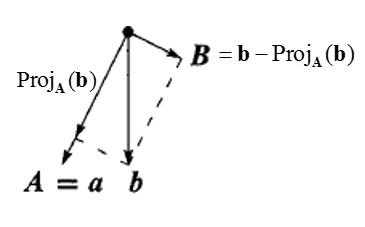
\includegraphics[width=5cm]{week5/gram}
\caption{Subtract projection to get $\bm B=\bm b-\Proj_{\bm A}\bm b$.}\label{figure_13.1}
\end{figure}
You can take inner product between $\bm A$ and $\bm B$ to verify that $\bm A$ and $\bm B$ are orthogonal in Figure (\ref{figure_13.1}). Note that $\bm B$ is not zero (otherwise $\bm a$ and $\bm b$ would be dependent. We will show it later.)
\item
Then we want to construct another vector $\bm C$. Most likely $\bm c$ is \emph{not} perpendicular to $\bm A$ and $\bm B$.  What we do is to \emph{subtract $\bm c$ off its projections onto the column space of $\bm A$ and $\bm B$ to get $\bm C$:}
\[
\text{\emph{Next Gram-Schmidt step}}\qquad\begin{aligned}
\bm C&=\bm c-\Proj_{\Span\{\bm A,\bm B\}}(\bm c)\\
&=\bm c-\Proj_{\bm A}(\bm c)-\Proj_{\bm B}(\bm c)\\
&=\bm c-\frac{\inp{\bm A}{\bm c}}{\inp{\bm A}{\bm A}}\bm A-\frac{\inp{\bm B}{\bm c}}{\inp{\bm B}{\bm B}}\bm B.
\end{aligned}
\]
\begin{figure}[H]\centering
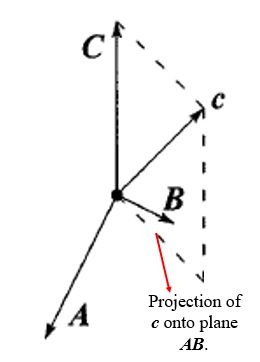
\includegraphics[width=5cm]{week5/nextgram}
\caption{Subtract $\bm c$ off its projections onto the column space of $\bm A$ and $\bm B$ to get $\bm C$}
\end{figure}
\item
Finally we get orthogonal vectors $\bm A,\bm B,\bm C$. Orthonormal vectors $\bm q_1,\bm q_2,\bm q_3$ are obtained by dividing their lengths (shown in Figure (\ref{Final_gram})):
\begin{figure}[H]\centering
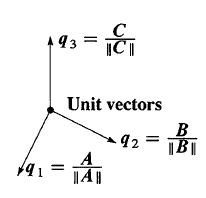
\includegraphics[width=5cm]{week5/finalgram}
\caption{Final Gram-Schmidt step}
\label{Final_gram}
\end{figure}
\end{itemize}
Next we show an example of Gram-Schmidt step:
\begin{example}
How to construct orthonormal vectors from 
\[
\begin{array}{lll}
\bm a=\begin{pmatrix}
1\\0\\1
\end{pmatrix},
&
\bm b=\begin{pmatrix}
1\\0\\0
\end{pmatrix},
&
\bm c=\begin{pmatrix}
2\\1\\0
\end{pmatrix}?
\end{array}
\]
\begin{itemize}
\item
Firstly we set $\bm A=\bm a=\begin{pmatrix}
1\\0\\1
\end{pmatrix}$.
\item
\[
\begin{aligned}
\bm B&=\bm b-\Proj_{\bm A}(\bm b)=\bm b-\frac{\inp{\bm A}{\bm b}}{\inp{\bm A}{\bm A}}\bm A\\
&=\begin{pmatrix}
1\\0\\0
\end{pmatrix}-\begin{pmatrix}
1\\0\\1
\end{pmatrix}\trans\begin{pmatrix}
1\\0\\0
\end{pmatrix}2^{-1}\begin{pmatrix}
1\\0\\1
\end{pmatrix}\\
&=\begin{pmatrix}
\frac{1}{2}\\0\\-\frac{1}{2}
\end{pmatrix}
\end{aligned}
\]
\item
\[
\begin{aligned}
\bm C&=\bm c-\Proj_{\bm A}(\bm c)-\Proj_{\bm B}(\bm c)=\bm c-\frac{\inp{\bm A}{\bm c}}{\inp{\bm A}{\bm A}}\bm A-\frac{\inp{\bm B}{\bm c}}{\inp{\bm B}{\bm B}}\bm B\\
&=\begin{pmatrix}
2\\1\\0
\end{pmatrix}-\begin{pmatrix}
1\\0\\1
\end{pmatrix}\trans\begin{pmatrix}
2\\1\\0
\end{pmatrix}2^{-1}\begin{pmatrix}
1\\0\\1
\end{pmatrix}-\begin{pmatrix}
\frac{1}{2}\\0\\-\frac{1}{2}
\end{pmatrix}\trans\begin{pmatrix}
2\\1\\0
\end{pmatrix}(\frac{1}{2})^{-1}\begin{pmatrix}
\frac{1}{2}\\0\\-\frac{1}{2}
\end{pmatrix}\\
&=\begin{pmatrix}
0\\1\\0
\end{pmatrix}
\end{aligned}
\]
Hence we obtain our orthonormal vectors:
\[
\bm q_1=\frac{\bm A}{\|\bm A\|}
=\begin{pmatrix}
\frac{1}{\sqrt 2}\\0\\\frac{1}{\sqrt 2}
\end{pmatrix},
,\bm q_2=\frac{\bm B}{\|\bm B\|}
=\begin{pmatrix}
\frac{1}{\sqrt 2}\\0\\-\frac{1}{\sqrt 2}
\end{pmatrix}
,\bm q_3=\frac{\bm C}{\|\bm C\|}
=\begin{pmatrix}
0\\1\\0
\end{pmatrix}
\]
\end{itemize}
And we derive the orthogonal matrix $\bm Q$:
\[
Q=\begin{pmatrix}
\frac{1}{\sqrt 2}&\frac{1}{\sqrt 2}&0\\0&0&1\\
\frac{1}{\sqrt 2}&-\frac{1}{\sqrt 2}&0
\end{pmatrix}
\]
\end{example}
When will the Gram-Schmidt process ``fail''? Let's describle this process in general case first, then we answer this question.
\subsubsection{Gram-Schmidt process in general case}
\emph{Algorithm: Gram-Schmidt Process}\\
\emph{Input: }a collection of vectors $\bm a_1,\dots,\bm a_n$, presumably linear independent.\\
Firstly construct orthogonal vectors $\bm A_1,\dots,\bm A_n$.

$\bm A_1=\bm a_1$.

To construct $\bm A_j$, $j\in\{2,\dots,n\}$, we compute $\bm a_j$ minus its projection in the column space spanned by $\{\bm A_1,\bm A_2,\dots,\bm A_{j-1}\}$:
\[
\begin{aligned}
\bm A_j&=\bm a_j-\Proj_{\Span\{\bm A_1,\bm A_2,\dots,\bm A_{j-1}\}}(\bm a_j)\\
&=\bm a_j-\Proj_{\bm A_1}(\bm a_j)-\Proj_{\bm A_2}(\bm a_j)-\dots-\Proj_{\bm A_{j-1}}(\bm a_j)\\
&=\bm a_j-\frac{\inp{\bm A_1}{\bm a_j}}{\inp{\bm A_1}{\bm A_1}}\bm A_1-\frac{\inp{\bm A_2}{\bm a_j}}{\inp{\bm A_2}{\bm A_2}}\bm A_2-\dots-\frac{\inp{\bm A_{j-1}}{\bm a_j}}{\inp{\bm A_{j-1}}{\bm A_{j-1}}}\bm A_{j-1}
\end{aligned}
\]
Secondly, after getting $\bm A_1,\dots,\bm A_n$, we can construct orthonormal vectors:
\[
\bm q_j=\frac{\bm A_j}{\|\bm A_j\|}\quad\text{for }j=1,2,\dots,n.
\]
So when do this process fail? When $\exists j$ such that $\bm A_j=\bm 0$, we cannot continue this process anymore:
\begin{proposition}
$\bm A_j\ne\bm0$ for $\forall j$ if and only if $\bm a_1,\bm a_2,\dots,\bm a_n$ are indendent.
\end{proposition}
\begin{proof}[Proofoutline.]
$\bm A_j=\bm0\Longleftrightarrow
\bm a_j=\Proj_{\Span{\{\bm A_1,\dots,\bm A_{j-1}\}}}(\bm a_j)$. It suffices to prove $\exists j$ s.t. $\bm A_j=\bm 0$ if and only if $\bm a_1,\bm a_2,\dots,\bm a_n$ are depependent.

\textit{Sufficiency. }Given $\bm A_j=\bm0$, then $\bm a_j=\Proj_{\Span{\bm A_1,\dots,\bm A_{j-1}}}(\bm a_j)\in\Span\{\bm A_1,\dots,\bm A_{j-1}\}$. It's easy to verify that $\Span\{\bm A_1,\dots,\bm A_{j-1}\}=\Span\{\bm a_1,\dots,\bm a_{j-1}\}$. Hence $\bm a_j\in\Span\{\bm a_1,\dots,\bm a_{j-1}\}$. Hence $\bm a_1,\dots,\bm a_j$ are dependent. Thus $\bm a_1,\dots,\bm a_n$ are dependent.

\textit{Necessity. }Given dependent vectors $\bm a_1,\dots,\bm a_n$, obviously, $\bm a_n\in\Span\{\bm a_1,\dots,\bm a_{n-1}\}$. It's easy to verify that $\bm a_n=\Proj_{\Span\{\bm  a_1,\dots,\bm a_{n-1}\}}(\bm a_n)$. Thus $\bm a_n=\Proj_{\Span\{\bm A_1,\dots,\bm A_{n-1}\}}(\bm a_n)\implies \bm A_n=\bm0$.
\end{proof}
\subsection[The Factorization $A=QR$.]{The Factorization $\bm A=\bm{QR}$}
We know that Gaussian Elimination leads to \textit{LU decomposition}; in fact, Gram-Schmidt process leads to \textit{QR factorization}. These two decomposition methods are quite important in Linear Algebra, let's discuss QR factorization briefly:
\begin{quotation}
Given a matrix $\bm A=\begin{bmatrix}
\bm a&\bm b&\bm c
\end{bmatrix}$, we finally end with a matrix $\bm Q=\begin{bmatrix}
\bm q_1&\bm q_2&\bm q_3
\end{bmatrix}$. How are these two matrices related?
\end{quotation}
\textit{Answer:} Since the linear combination of $\bm a,\bm b,\bm c$ leads to $\bm q_1,\bm q_2,\bm q_3$ (vice versa), there must be a third matrix connecting $\bm A$ to $\bm Q$. This third matrix is the triangular $\bm R$ such taht $\bm A=\bm{QR}$.

Let's discuss a specific example to show how to do QR factorization.
\begin{example}
Given $\bm A=\begin{bmatrix}
\bm a&\bm b&\bm c
\end{bmatrix}$, whose columns are independent, then we can use Gram-Schmidt process to obtain the corresponding orthonormal vectors $\bm q_1,\bm q_2,\bm q_3$ from $\bm a,\bm b,\bm c$. As a result,
we can write $\bm A$ as:
\[
\bm A=\begin{bmatrix}
\bm q_1&\bm q_2&\bm q_3
\end{bmatrix}\begin{bmatrix}
\bm q_1\trans\bm a&\bm q_1\trans\bm b&\bm q_1\trans\bm c\\0&\bm q_2\trans\bm b&\bm q_2\trans\bm c\\0&0&\bm q_3\trans\bm c
\end{bmatrix}
\]


We define $\bm R\triangleq\begin{bmatrix}
\bm q_1\trans\bm a&\bm q_1\trans\bm b&\bm q_1\trans\bm c\\0&\bm q_2\trans\bm b&\bm q_2\trans\bm c\\0&0&\bm q_3\trans\bm c
\end{bmatrix}, \bm Q\triangleq\begin{bmatrix}
\bm q_1&\bm q_2&\bm q_3
\end{bmatrix}$.

Hence $\bm A$ could be factorized into:
\[
\bm A=\bm{QR}
\]
where $\bm R$ is upper triangular, $\bm Q$ is a matrix with orthonormal columns.
\end{example}
QR factorization holds for every matrix with independent columns:
\begin{theorem}
Every $m\times n$ matrix $\bm A$ with ind. columns can be factorized as
\[
\bm A=\bm{QR}
\]
where $\bm Q$ is a matrix with \textit{orthonormal columns}, $\bm R$ is an upper triangular matrix (always square).
\end{theorem}
We omit the proof of this theorem. Now we show that the inverse of $\bm R$ always exists:
\begin{proof}
suppose $\bm A=\begin{bmatrix}
\bm a_1&\bm a_2&\dots&\bm a_n
\end{bmatrix}, \bm Q=\begin{bmatrix}
\bm q_1&\bm q_2&\dots&\bm q_n
\end{bmatrix}$.
 Thus we derive \[\bm R=\bm Q^{-1}\bm A=\bm Q\trans\bm A=\begin{bmatrix}
\bm q_1\trans\bm a_1&\bm q_1\trans\bm a_2&\dots&\bm q_1\trans\bm a_n\\
0&\bm q_2\trans\bm a_2&\dots&\bm q_2\trans\bm a_n\\
\vdots&\vdots&\ddots&\vdots\\
0&0&\dots&\bm q_n\trans\bm a_n
\end{bmatrix}
\]
For every step $j$ we have 
\[\bm A_j=\bm a_j-\Proj_{\Span\{a_1,\dots,a_{j-1}\}}( \bm a_j),\qquad \bm q_j=\frac{\bm A_j}{\|\bm A_j\|}.
\]
Since $\inp{\bm A_j}{\bm a_j}=\inp{\bm a_j}{\bm a_j}-\inp{\Proj_{\Span\{a_1,\dots,a_{j-1}\}}(\bm a_j)}{\bm a_j}=\|a_j\|^2-\|\Proj_{\Span\{a_1,\dots,a_{j-1}\}}(\bm a_j)\|^2>0$, we have $\inp{\bm q_j}{\bm a_j}=\frac{\inp{\bm A_j}{\bm a_j}}{\|\bm A_j\|}>0.$ Hence the diagonal of $\bm R$ are all positive. Hence this triangular matrix is \textit{invertible.}
\end{proof}
\begin{proposition}
If $\bm A=\bm{QR}$, then the least squares solution is given by: 
\[
\bm x=(\bm R\trans\bm R)^{-1}\bm R\trans\bm Q\trans\bm b=\bm R^{-1}\bm Q\trans\bm b.
\]
\end{proposition}
\begin{proof}[Explain:]
Since we have
\[
\begin{aligned}
\bm A\trans\bm A\bm x&=\bm R\trans\bm Q\trans\bm Q\bm R\bm x=\bm R\trans\bm R\bm x\\
\bm A\trans\bm b&=\bm R\trans\bm Q\trans\bm b
\end{aligned}
\]
it's equivalent to solve $\bm R\trans\bm R\bm x=\bm R\trans\bm Q\trans\bm b$.\\
Sicne $\bm R$ is \textit{invertible}, we solve by back substitution to get
\[
\bm x=(\bm R\trans\bm R)^{-1}\bm R\trans\bm Q\trans\bm b=\bm R^{-1}\bm Q\trans\bm b.
\]
\end{proof}
\subsection{Function Space}
Sometimes we may also discuss orthonormal basis and Gram-Schmidt process on function space. There is a simple example:
\begin{example}
For subspace $\Span\{1,x,x^2\}\subset \mathcal{C}[-1,1]$, firstly, how to define orthogonal for the basis $\{1,x,x^2\}$?

\textit{Pre-requisite Knowledge: }Inner product.
\[
\inp{f}{g}=\int_{a}^{b}fg\diff x \text{ for $f,g\in C[a,b]$.}\qquad
\|f\|^2=\int_{a}^{b}f^2\diff x
\]
If we have defined inner product, then we can talk about \textit{orthogonality} for $\{1,x,x^2\}$. It's easy to verify that
\[
\inp{1}{x}=0\quad\inp{x}{x^2}=0\quad\inp{1}{x^2}=\frac{2}{3}.
\]
If we do the Gram-Schmidt Process similarly, we obtain:
\[
\bm A=1,\qquad\bm B=x,\qquad
\bm C=x^2-\frac{\inp{1}{x^2}}{\inp{1}{1}}1-\frac{\inp{x}{x^2}}{\inp{x}{x}}x=x^2-\frac{1}{3}
\]
where $\bm A,\bm B,\bm C$ are \textit{orthogonal}. We can divide their length to obtain orthonormal basis:
\[
\begin{aligned}
\bm q_1&=\frac{\bm A}{\|\bm A\|}=\frac{1}{\sqrt{\int_{-1}^{1}1^2\diff x}}=\frac{1}{2}\qquad\\
\bm q_2&=\frac{\bm B}{\|\bm B\|}=\frac{x}{\sqrt{\int_{-1}^{1}x^2 \diff x}}=\frac{x}{2/3}=\frac{3}{2}x\qquad\\
\bm q_3&=\frac{\bm C}{\|\bm C\|}=\frac{x^2-\frac{1}{3}}{\sqrt{\int_{-1}^{1}(x^2-\frac{1}{3})^2 \diff x}}=\frac{x^2-\frac{1}{3}}{\frac{8}{45}}=\frac{45x^2-15}{8}
\end{aligned}
\]
Hence $\{\bm q_1,\bm q_2, \bm q_3\}$ is the orthonormal basis for $\{1,x,x^2\}$.
\end{example}
\begin{example}\label{Exp:6:11}
Consider the collection $\mathcal{F}$ of functions defined on $[0,2\pi]$, where
\[
\mathcal{F}:=\{1,\cos x,\sin x,\cos 2x,\sin 2x,\dots,\cos mx,\sin mx,\dots\}
\]
Using various trigonometric identities, we can show that if $f$ and $g$ are \emph{distinct}(different) functions in $\mathcal{F}$, we have $\int_{0}^{2\pi}fg\diff x=0$. For example,
\[
\inp{\sin x}{\sin 2x}=\int_{0}^{2\pi}\sin x\sin 2x\diff x=\int_{0}^{2\pi}\frac{1}{2}(\cos x-\cos 3x)\diff x=0.
\]
And moreover, if $f=g$, we have $\int_{0}^{2\pi}f^2\diff x=\pi$. For example,
\[
\inp{\sin 5x}{\sin 5x}=\int_{0}^{2\pi}\sin^2 5x\diff x=\int_{0}^{2\pi}\frac{1}{2}(1+\cos 10x)\diff x=\pi.
\]
In conclusion, the collection of functions $\{1,\sin mx,\cos mx\}$ for $k=1,2,\dots$ are \textit{orthogonal} in $\mathcal{C}[0,2\pi]$. Note that this set is \emph{not orthonormal}.
\end{example}
This example gives a motivation of the fourier transformation:
\subsection{Fourier Series}
Since we have shown the orthogonality of $\mathcal{F}$ in Example.(\ref{Exp:6:11}), our question is that what kind of function can be written as the linear combination of functions from $\mathcal{F}$.

The Fourier series of a function is its expansion into sines and cosines:
\[
f(x)=a_0+a_1\cos x+b_1\sin x+a_2\cos 2x+b_2\sin 2x+\dots
\]
where $f(x)\in \mathcal{C}[0,2\pi]$. So our question turns into what kind of function could be expressed as fuourier series?
\begin{theorem}
If a function $f$ have the finite length in its function space $\mathcal{C}[a,b]$, then it could be expressed as \textit{fourier series}.
\end{theorem}
But how to compute the coefficients $a_i's$ and $b_j's$? The key is orthogonality! For example, in order to get $a_1$, we just do the inner product between $f(x)$ and $\cos x$:
\begin{figure}[H]\centering
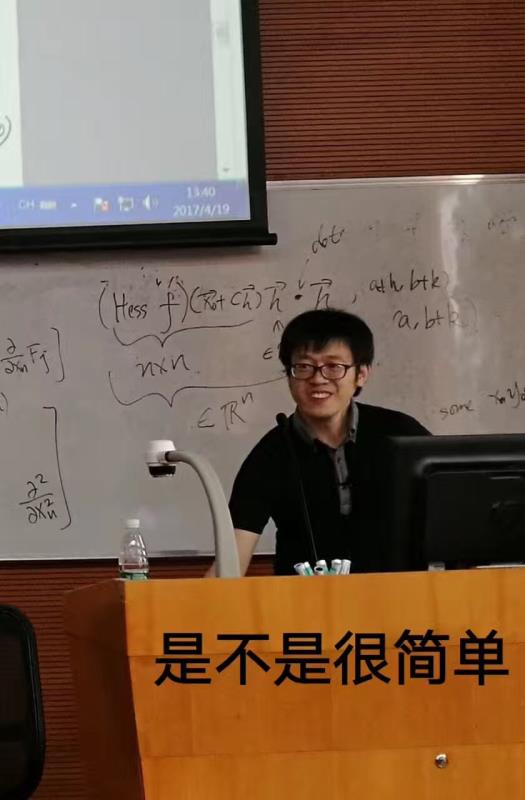
\includegraphics[width=3cm]{week5/1810645243}
\caption{Enjoy fourier series!}
\end{figure}
\[
\inp{f(x)}{\cos x}=a_1\inp{\cos x}{\cos x}+0
\implies
a_1=\frac{\inp{f(x)}{\cos x}}{\inp{\cos x}{\cos x}}=\frac{1}{\pi}\int_{0}^{2\pi}f(x)\cos x\diff x
\]
Similarly we derive 
\[
a_m=\frac{1}{\pi}\int_{0}^{2\pi}f(x)\cos mx\diff x
\qquad
b_m=\frac{1}{\pi}\int_{0}^{2\pi}f(x)\sin mx\diff x.
\]